\chapter{High-energy nuclear physics}
\section{Quantum Chromodynamics}
In the mid-20$^{\mathrm{th}}$ century, the realm of particle physics underwent a transformative phase, marked by the discovery of a seemingly endless variety of subatomic particles. This era witnessed the unveiling of numerous mesons and baryons, which left physicists with the necessity of developing a framework that could describe the behaviour of these particles and their interactions. This led to the development of the static quark model, which emerged in the 1960s as a groundbreaking conceptual framework to categorize the various observed particles. Developed independently by Murray Gell-Mann\cite{Gell-Mann:1964ewy} and George Zweig\cite{Zweig:1964jf, Fritzsch:1972jv}, this model postulated the existence of fundamental constituents called quarks, which, in order to reflect the experimental findings, had to be fermions (to describe baryons with spin 1/2 and 3/2) with fractional electric charge. The quark model beautifully explained the organization of hadrons in terms of three quarks ($u$, $d$, and $s$), leading to the development of a more structured and coherent classification of particles.

Despite the phenomenological success of the static quark model, it had two problems: it introduced particles with fractional charge, which had never been observed before, and, most importantly, it gave rise to a violation of the Fermi-Dirac statistics. The $\Delta^{++}$, $\Delta^{-}$, and $\Omega^{-}$ baryons, in fact, have symmetric orbital, spin and flavour wavefunctions, which defied the Pauli exclusion principle that should have implied antisymmetric wavefunctions for these particles.

To resolve these inconsistencies, a new degree of freedom, the \emph{colour}, was introduced. Hadrons wavefunctions were assumed to be totally antisymmetric in colour quantum numbers, effectively implementing the Pauli exclusion principle.

The simplest model of colour would be to assign quarks to the fundamental representation of a global $SU(3)$ symmetry. Each quark now carries a colour index: $q_i$, where $i = 1, 2, 3$, and transforms under the fundamental ($3$) representation of $SU(3)$, while antiquarks,  $\bar{q}_i$, transform in the $\bar{3}$ representation. Introducing the totally antisymmetric tensor $\varepsilon^{ijk}$, possible compositions of quarks that give rise to colour singlets are 
\begin{equation*}
    \bar{q}^iq_i,\qquad \varepsilon^{ijk}q_iq_jq_k,\qquad \varepsilon^{ijk}\bar{q_i}\bar{q_j}\bar{q_k},
\end{equation*}
which are the quarks compositions of mesons, baryons, and antibaryons, respectively. 

One of the tests supporting the existence of colour and fractional electric charge came in the form of the ratio R, of the $\mathrm{e}^+ \mathrm{e}^-$ total hadronic cross-section to the cross-section of a pair of muons produced from the same annihilation process. The virtual photon emitted in the annihilation can produce all electrically charged pairs of particles and antiparticles, as shown in Fig.~\ref{fig:ee_to_ff_diagram}.

\begin{figure}[h]
    \centering
        \feynmandiagram [horizontal=a to b] {
          i1 [particle=\(e^{-}\)] -- [fermion] a -- [fermion] i2 [particle=\(e^{+}\)],
          a -- [photon, edge label=\(\gamma^*\)] b,
          f1 [particle=\(\bar{f}\)] -- [fermion] b -- [fermion] f2 [particle=\(f\)],
        };
\caption{$\mathrm{e}^+ \mathrm{e}^-$ annihilation to a pair of fermions}
    \label{fig:ee_to_ff_diagram}
\end{figure}


The ratio R is given by:
\begin{equation*}
    R = \frac{\sigma(e^+e^- \rightarrow hadrons)}{\sigma(e^+e^- \rightarrow \mu^+\mu^-)} = N_c \sum_f Q_f^2\ ,
\end{equation*}
where $N_c$ represents the number of existing colours and $Q_f$ is the electric charge of the quark flavour $f$. Notably, this ratio is dependent on the energy of the center-of-mass system and encompasses all possible quark flavors that can be produced by the virtual photon at that specific energy level. The experimental data for $R$ (shown in Fig.~\ref{fig:R_vs_s}) exhibited a remarkable agreement with the predictions of the three-color model, thereby providing compelling evidence for the existence of color and fractional electric charge of quarks.

The final step that propelled the development of QCD as a comprehensive theory of the strong force was the insight into the mechanism that ensured all hadron wavefunctions to be color singlets. This emerged from the discovery of asymptotic freedom, a phenomenon observed in deep-inelastic scattering experiments. Non-Abelian gauge theories, often referred to as Yang-Mills theories, were identified as having this unique characteristic. This realization led to the formulation of QCD by elevating the global color $SU(3)$ symmetry to a local one, allowing the 8 quanta of the $SU(3)$ gauge field, called \emph{gluons}, to mediate the strong force, successfully describing the confinement and behavior of quarks and gluons within hadrons.

\begin{figure}[p]
    \centering
    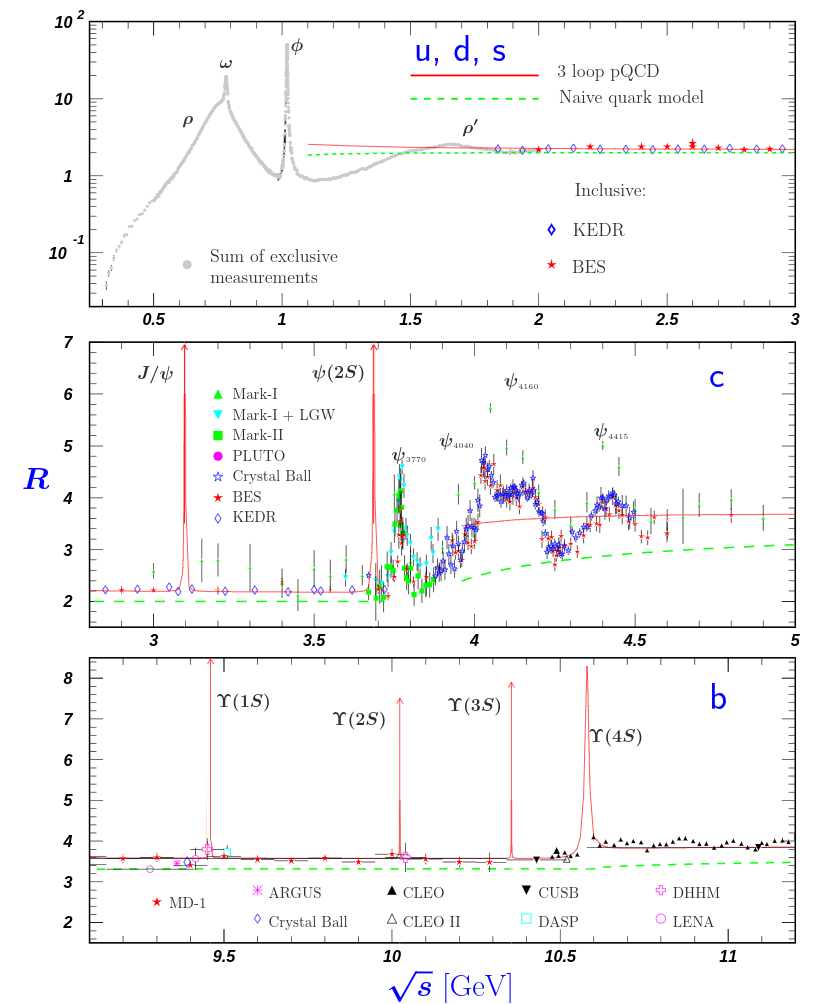
\includegraphics[width=\linewidth]{Figures/Chapter 1/rpp2022-R_udscb.pdf}
    \caption{$R$ as a function of $\sqrt{s}$ in the light-flavor, charm, and beauty threshold regions taken from \cite{pdg}. The green curve is a naive quark-parton model prediction, while the red one is a 3-loops pQCD prediction. Breit-Wigner parameterizations of $J/\psi$, $\psi$(2S), and $\Upsilon$(nS), n = 1,2,3,4 are also shown}
    \label{fig:R_vs_s}
\end{figure}

The QCD Lagrangian density can be written as:
\begin{equation}\label{eq:Lqcd}
    \mathcal{L}_{QCD}=-\frac{1}{4} F^a_{\mu\nu}F_a^{\mu\nu} + \sum_f \bar{q}_f^i (i\gamma^\mu(\mathcal{D}_\mu)_{ij}-m_f\delta_{ij})q_f^j\ ,
\end{equation}
where $F^a_{\mu\nu}$ is the field strength tensor defined in terms of the gluon field $A^a_\mu$ and the $SU(3)$ structure constant $f^{abc}$:
\begin{equation} \label{eq:F}
    F^a_{\mu\nu} = \partial_\mu A^a_\nu - \partial_\nu A^a_\mu + g_s f^{abc}A^b_\mu A^c_\nu 
\end{equation}
and $(\mathcal{D}_\mu)_{ij}$ is the covariant derivative:
\begin{equation*}
    (\mathcal{D}_\mu)_{ij} = \partial_\mu \delta_{ij} - ig_s(t^a)_{ij}A_\mu^a\ ,
\end{equation*}
with $t^a$ being one of the generators of the $SU(3)$ representation.

The last term in Eq.~\ref{eq:F} is peculiar to non-Abelian theories, and gives rise to triplet and quartic gluon self-interactions illustrated in Fig.~\ref{fig:Feynman-gluons}. $g_s$ is the coupling constant, which determines the strength of the interaction between the coloured particles.

\begin{figure}[htb]
    \centering
    \begin{tikzpicture}
      \begin{feynman}
        \vertex (a) {a};
        \vertex [right=of a] (b);
        \vertex[above right= of b] (c) {b};
        \vertex[below right= of b] (d) {c};
        \diagram* {
          (a) -- [gluon] (b),
          (b) -- [gluon] (c),
          (b) -- [gluon] (d),
        };
      \end{feynman}
    \end{tikzpicture} \qquad
    \begin{tikzpicture}
      \begin{feynman}
        \vertex (a);
        \vertex[above left=of a] (b) {a};
        \vertex[above right= of a] (c) {b};
        \vertex[below right= of a] (d) {c};
        \vertex[below left= of a] (e) {d};
        \diagram* {
          (a) -- [gluon] (b),
          (a) -- [gluon] (c),
          (a) -- [gluon] (d),
          (a) -- [gluon] (e),
        };
      \end{feynman}
    \end{tikzpicture}
    \caption{Feynman diagrams for gluons self-interactions}
    \label{fig:Feynman-gluons}
\end{figure}

The second term of Eq.~\ref{eq:Lqcd} describes the interactions between quarks and gluons, sketched in Fig.~\ref{fig:Feynman_q_g}, and contains the mass term for the fermions. It is noteworthy to observe that the interaction between quarks and gluons is diagonal in flavor, meaning that the strong interaction conserves the flavor of quarks. In contrast, colour mixing is allowed within the framework of QCD.

\begin{figure}[htb]
    \centering
    \begin{tikzpicture}
      \begin{feynman}
        \vertex (a);
        \vertex [below=0.1em of a] {$t^a_{ij}$};
        \vertex[left=of a] (b) {$q_i$};
        \vertex[right= of a] (c) {$q_j$};
        \vertex[above right= of a] (d) {a};
        \diagram* {
          (b) -- [fermion] (a),
          (a) -- [fermion] (c),
          (a) -- [gluon] (d),
        };
      \end{feynman}
    \end{tikzpicture}
    \caption{Feynman diagram for quark-gluon interaction}
    \label{fig:Feynman_q_g}
\end{figure}

\subsection{Running coupling constant}
If one considers a dimensionless physical observable, denoted in the following as $R$, which solely depends on a single energy scale, $Q$, one might naturally expect that $R$ would maintain a constant value, independent of the specific energy scale chosen. However, this does not hold true when loop diagrams are studied: the necessity of renormalisation introduces a new energy scale denoted as $\mu$. This scale, known as the renormalisation scale, is the point at which the subtraction of the ultraviolet divergences is carried out. Critically, $\mu$ is an arbitrary parameter and, as such, is non-physical. Consequently, $R$ becomes dependent on the ratio $Q^2/\mu^2$ and the renormalised coupling $\alpha_s = g_s^2/4\pi$: $R = R\left(\frac{Q^2}{\mu^2},\als\right)$. The $\mu$ independence of $R$ (which is an essential requirement given $\mu$'s arbitrariness) can be expressed as:
\begin{equation}\label{eq:RGE}
    \mu^2 \frac{\de R\left(\frac{Q^2}{\mu^2},\alpha_s\right)}{\de \mu^2} = \mu^2 \left[\frac{\partial}{\partial\mu^2}+\frac{\partial \alpha_s}{\partial\mu^2}\frac{\partial}{\partial\alpha_s}\right]R\left(\frac{Q^2}{\mu^2},\alpha_s\right) = 0\ , 
\end{equation}
a fundamental equation known as the renormalisation group equation. This equation is exactly true in the case of a prediction that considers all perturbative orders. If one limits the expansion at a fixed order $\alpha_s^N$, then a dependence of $R$ from $\mu$ is observed at the $\als^{N+1}$ order.\\ Solving Eq.~\ref{eq:RGE} requires the introduction of the concept of the running coupling $\alpha_s(Q^2)$, which evolves as a function of $Q$. By introducing
\begin{equation*}
    t\equiv \mathrm{log}(Q^2/\mu^2), \qquad \beta(\als)\equiv \mu^2 \frac{\de\als}{\mathrm{\mu^2}}\quad ,
\end{equation*}
Eq.~\ref{eq:RGE} can be written as
\begin{equation*}
    \left(-\frac{\partial}{\partial t} + \beta(\als)\frac{\partial}{\partial \als}\right) R(e^t,\als) = 0
\end{equation*}
This first-order partial differential equation can be solved by defining a new function: the running coupling $\als(Q^2)$
\begin{equation}\label{eq:t_integral}
    t = \mathrm{log}(Q^2/\mu^2) \equiv \int_{\als}^{\als(Q^2)} \frac{\de x}{\beta(x)} , \quad \mathrm{with}~\als=\als(\mu^2)\quad .
\end{equation}
By differentiating Eq.~\ref{eq:t_integral} with respect to $t$ and \als, one gets:
\begin{equation}\label{eq:beta_def}
    \beta(\als(Q^2)) = \frac{\partial\als(Q^2)}{\partial t}, \quad \frac{\de\als(Q^2)}{\de\als} = \frac{\beta(\als (Q^2))}{\beta(\als)}\quad .
\end{equation}
It results from this last set of equations that $R(1,\als(Q^2))$ satisfies Eq.~\ref{eq:RGE}; hence, the running coupling constant has absorbed the $\mu$ scale dependence of $R$. As a consequence, the knowledge of $R(1,\als)$, which can be evaluated in fixed-order perturbation theory, allows to know the dependence of $R$ from $Q^2$, which is the physical scale at which the coupling is gauged, by simply substituting $\als \rightarrow \als(Q^2)$. 

\subsubsection{The \ensuremath{\beta} function}
The running of the coupling constant is determined by the $\beta(\als)$ function, which is evaluated from loop corrections to the bare vertices of the theory. As of the time of the writing of this Thesis, the $\beta$ function has been evaluated up to 5 loops\cite{Herzog:2017ohr}. In Fig.~\ref{fig:beta_loops}, the 1-loop Feynman diagrams contributing to the $\beta$ function evaluation are reported.

\begin{figure}[htb]
    \centering
    \begin{tikzpicture}
      \begin{feynman}
        \vertex (a);
        \vertex [right=1cm of a] (b);
        \vertex[right=1cm of b] (c);
        \vertex[right=1cm of c] (d);
        \diagram* {
            (a) -- [gluon] (b)
            -- [fermion, half left, looseness=1.5] (c)
            -- [fermion, half left, looseness=1.5] (b),
            (c) -- [gluon] (d),
        };
      \end{feynman}
    \end{tikzpicture}\quad
    \begin{tikzpicture}
      \begin{feynman}
        \vertex (a);
        \vertex [right=1cm of a] (b);
        \vertex[right=1cm of b] (c);
        \vertex[right=1cm of c] (d);
        \diagram* {
            (a) -- [gluon] (b)
            -- [gluon, half left, looseness=1.5] (c)
            -- [gluon, half left, looseness=1.5] (b),
            (c) -- [gluon] (d),
        };
      \end{feynman}
    \end{tikzpicture}\quad
    \begin{tikzpicture}
      \begin{feynman}
        \vertex (a);
        \vertex [right=of a] (b);
        \vertex[above=1cm of b] (c);
        \vertex[right=of b] (d);
        \diagram* {
            (a) -- [gluon] (b)
            -- [gluon, half left, looseness=1.5] (c)
            -- [gluon, half left, looseness=1.5] (b),
            (b) -- [gluon] (d),
        };
      \end{feynman}
    \end{tikzpicture}\quad

    \vspace{0.6cm}
    \begin{tikzpicture}
      \begin{feynman}
        \vertex (a);
        \vertex [right=1cm of a] (b);
        \vertex[right=1cm of b] (c);
        \vertex[right=1cm of c] (d);
        \diagram* {
            (a) -- [gluon] (b)
            -- [ghost, half left, looseness=1.5] (c)
            -- [ghost, half left, looseness=1.5] (b),
            (c) -- [gluon] (d),
        };
      \end{feynman}
    \end{tikzpicture}\quad
    \begin{tikzpicture}
      \begin{feynman}
        \vertex (a);
        \vertex [right=1cm of a] (b);
        \vertex[right=1cm of b] (c);
        \vertex[right=1cm of c] (d);
        \vertex[below=0.31cm of c] (f) {$ $};
        \diagram* {
            (a) -- [fermion] (b) -- [fermion] (c) -- [fermion] (d),
            (b) -- [gluon, half left, looseness=1.5] (c)
            
        };
      \end{feynman}
    \end{tikzpicture}\quad
    
    \vspace{0.5cm}
    \begin{tikzpicture}
      \begin{feynman}
        \vertex (a);
        \vertex [right=1cm of a] (b);
        \vertex[above right=1cm of b] (c);
        \vertex[right=1cm of c] (d);
        \vertex[below right=1cm of b] (e);
        \vertex[right=1cm of e] (f);
        \diagram* {
            (a) -- [gluon] (b) -- [fermion] (c) -- [fermion] (d),
            (b) -- [fermion] (e) -- [fermion] (f),
            (c) -- [gluon] (e)
        };
      \end{feynman}
    \end{tikzpicture}\quad
    \begin{tikzpicture}
      \begin{feynman}
        \vertex (a);
        \vertex [right=1cm of a] (b);
        \vertex[above right=1cm of b] (c);
        \vertex[right=1cm of c] (d);
        \vertex[below right=1cm of b] (e);
        \vertex[right=1cm of e] (f);
        \diagram* {
            (a) -- [gluon] (b) -- [gluon] (c),
            (b) -- [gluon] (e),
            (f) -- [fermion] (e) -- [fermion] (c) -- [fermion] (d)
        };
      \end{feynman}
    \end{tikzpicture}\quad
    \caption{1-loop Feynman diagrams contributing to the $\beta$ function evaluation}
    \label{fig:beta_loops}
\end{figure}

By limiting the calculations at the first order in the perturbative expansion, one gets:
\begin{equation}\label{eq:beta0}
    \beta(\als) = -\als^2 \frac{11 \mathrm{N_c} - 2 \mathrm{N_f}}{12\pi} + \mathcal{O}(\als^3) \equiv -\als^2 \beta_0 + \mathcal{O}(\als^3)\quad ,
\end{equation}
where $\mathrm{N_c}$ is the number of colours (3), while $\mathrm{N_f}$ is the number of quark flavours which can be considered massless at the physical scale $Q^2$ at which the coupling is being measured.
From Eqs.~\ref{eq:beta0} and \ref{eq:beta_def}, one can extract the $Q^2$ dependency of the running coupling constant:
\begin{equation}\label{eq:alpha_s_running}
    \alpha_s(Q^2) = \frac{\alpha_s(\mu^2)}{1+\alpha_s(\mu^2)\beta_0 \mathrm{log}(Q^2/\mu^2)}\ ,
\end{equation}
Notably, since $\beta_0$ is positive also when considering 6 quark flavours, the strong coupling constant exhibits a monotonic decreasing trend as a function of $Q^2$. This behaviour differs from the one of the electromagnetic coupling constant, which increases with the energy scale due to the screening effect of vacuum polarisation. For QCD, the running of the coupling constant is a direct consequence of the non-Abelian nature of the theory, allowing for gluon self-interactions, which give rise to an anti-screening effect. The idea is that the emission of virtual gluons by static colour sources causes their colour charges to 'leak out' into the surrounding vacuum. Since the interaction between distributions of charges is weaker than the one between point-like charges when the distributions overlap, the effective coupling constant decreases at short distances. This behaviour is known as asymptotic freedom, a key feature of QCD that allows for the perturbative expansion of the theory at high energy scales, where the strong coupling constant is small. At the same time, the running of the coupling constant implies that the theory is non-perturbative at low energy scales, and phenomenological models are required to describe the strong interaction in this regime. Instead of using the renormalisation scale $\mu$ as a free parameter, one can use the running coupling constant to define a physical scale, $\Lambda_{QCD}$, which is the energy scale at which the coupling constant would diverge, if extrapolated outside the perturbative regime. Using Eq.~\ref{eq:alpha_s_running}, one can write:
\begin{equation*}
    \alpha_s(\Lambda_{QCD}) = \frac{1}{\beta_0 \mathrm{log}(Q^2/\Lambda_{QCD}^2)}\quad .
\end{equation*}
The value of $\Lambda_{QCD}$ is determined by its specific definition. However, to obtain the value of the coupling constant measured at $Q^2 = M_Z^2$, an approximate value of $\Lambda_{QCD}$ is around 200 MeV.

Measurements of the running of the coupling constant at different values of $Q$ are illustrated in Fig.~\ref{fig:alpha_s_running} and compared to the theoretical prediction at 5 loops. The agreement between the experimental data and the theoretical prediction is remarkable, confirming the validity of the QCD framework at high energy scales.


\begin{figure}[htb]
    \centering
    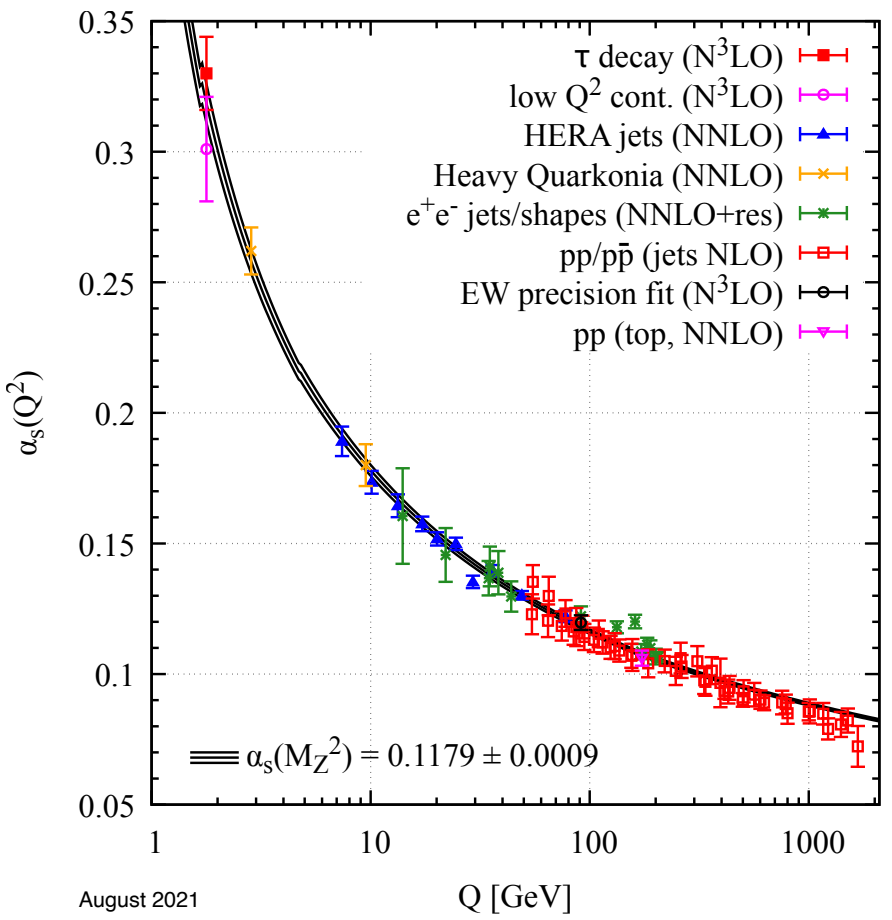
\includegraphics[width=0.7\linewidth]{Figures/Chapter 1/Alpha_s_running.png}
    \caption{Summary of measurements of \als as a function of the energy scale $Q$, compared to the running of the coupling computed at five loops, taking as an input the current PDG average, $\als(M_Z^2) = 0.1180 \pm 0.0009$ \gevcc.}
    \label{fig:alpha_s_running}
\end{figure}

\section{Confinement}
The concept of confinement is one of the most intriguing aspects of QCD. It is the phenomenon by which quarks and gluons are never observed as free particles, but are always confined within colour-neutral hadrons. The confinement of quarks and gluons is a direct consequence of the non-Abelian nature of the theory, which, as described in the previous Section, is characterised by an increase of the strong coupling constant at low energy scales. This leads to the formation of colour-neutral hadrons, which are the only particles that can be observed in nature. The confinement of quarks and gluons is a non-perturbative effect, and the theoretical description of this phenomenon is still an open question in QCD. Some phenomenological models, such as the MIT bag model, have been proposed to describe confinement, but a complete understanding of this phenomenon is still lacking. Lattice QCD simulations are the most successful approach to study the non-perturbative regime of the theory, and they have provided a wealth of information on the properties of hadrons and the strong interaction at low energy scales.

\subsection{MIT bag model}
The MIT bag model~\cite{Johnson:1975zp} is a phenomenological model of confinement, which describes hadrons as bound states of quarks and gluons confined within a finite volume, called the bag. The model was developed in the 1970s by A. Chodos, R. L. Jaffe, K. Johnson, C. B. Thorn, and V. F. Weisskopf, and it has been widely used to study the properties of hadrons and the strong interaction. In the MIT bag model, N masslesss fermions are confined within a spherical cavity of radius $R$, which is the bag radius. The confinement arises from a balance between pressure due to the kinematic energy of the fermions inside the bag and an ad hoc external pressure, which is introduced to confine the fermions within the bag. The fermions are described by the Dirac equation for massless fermions:

\begin{equation*}
    i\gamma^\mu\partial_\mu\psi = 0\quad ,
\end{equation*}
where $\psi$ is the fermion field, and $\gamma^\mu$ are the Dirac matrices. The solution to the Dirac equation is given in terms of the spherical Bessel functions of the zeroth and first order, $j_0(p_0r)$ and $j_1(p_0r)$, where $p_0$ is the energy of the fermion:

\begin{equation*}
    \psi = \mathcal{N} e^{-ip_0t} \begin{pmatrix} j_0(p_0r)\chi^+ \\ \vec{\sigma}\cdot\hat{r}j_1(p_0r)\chi^-\end{pmatrix}\quad ,
\end{equation*}
where $\chi^+$ and $\chi^-$ are the two components of the fermion four dimentional spinor $\psi$, and $\vec{\sigma}$ are the Pauli matrices. The colour flux at a point $r$ inside the bag is given by:

\begin{equation*}
    j_{ab}^\mu(r) = \bar{\psi_a}(r)\gamma^\mu\psi_b(r)\quad ,
\end{equation*}
where $a$ and $b$ are the colour indices of the fermions. If the quantum numbers are not to be lost through the surface of the bag, which is the definition of confinement, then:

\begin{equation*}
  n_\mu j_{ab}^\mu(r) = \bar{\psi_a}(r)\gamma\cdot n \psi_b(r) = 0\quad ,
\end{equation*}
on the surface, where $n$ is a unit space-like vector normal to the surface. Using the gamma properties, $(i\gamma\cdot n)^2 = 1$, so that by assuming that $i\gamma\cdot n = + 1$, the boundary condition on the surface of the bag is given by:

\begin{equation*}
    \bar{\psi}(R)\psi(R) = 0\quad ,
\end{equation*}
leading to the solution of the Dirac equation in the bag:

\begin{equation*}
    \left[j_0\left(p_0R\right)\right]^2 - \left[j_1\left(p_0R\right)\right]^2 = 0\quad ,
\end{equation*}
with solution $p_0R = 2.04$. The total energy inside the bag is given by:

\begin{equation*}
    E = \frac{2.04 N}{R}(\hbar c) + \frac{4\pi}{3}R^3B\quad ,
\end{equation*}
where the first term is the kinetic energy of the fermions, and the second term is the energy due to the presence of an external pressure $B$ which keeps the fermions confined in the bag. The bag pressure is a phenomenological parameter of the model, and it is introduced to confine the fermions within the bag. It can be extracted by minimising the energy of the system with respect to the bag radius $R$, yielding $B=234$ MeV/fm$^3$, for a baryon with $R=0.8$ fm.

\subsection{Lattice QCD}
Lattice QCD is a numerical technique used to study the non-perturbative regime of QCD. The method is based on the discretisation of spacetime on a four-dimensional lattice, and the evaluation of the path integral of the theory by Monte Carlo methods, i.e. by sampling possible configurations of the quark and gluon fields according to the probability distribution given by the QCD Lagrangian. The lattice spacing is a parameter of the method, and allows one to avoid the ultraviolet divergences of the theory, which are typical in perturbative QCD, by introducing a cutoff on the momenta of the quark and gluon fields. 
\begin{figure}[htb]
  \centering
  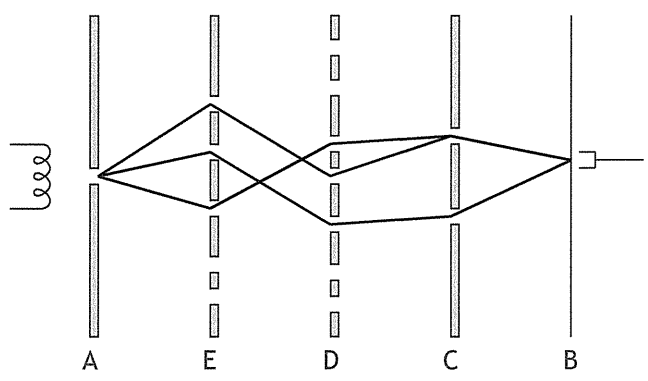
\includegraphics[width=0.7\linewidth]{Figures/Chapter 1/PathIntegrals.png}
  \caption{Feynman introduction to path integrals. Here, a particle emitted from a source at $x_a$ is detected at $x_b$. A finite number of screens, each with a finite number of holes, is placed between the source and the detector. The probability amplitude for the particle to hit the detector is given by the sum of the probabilities of moving from the source to the detector through all possible paths. By adding an infinite amount of screens with an infinite number of holes, and by also considering the time at which the particle passes through the screens, the sum becomes an integral over all possible paths, called a \emph{path integral}.}
  \label{fig:PathIntegrals}
\end{figure}
The Lattice QCD simulations are based on the path integral formalism of quantum field theory~\cite{RevModPhys.20.367}, developed by R. Feynman in the 1940s. The path integral provides a natural extension of the least action principle of classical mechanics to quantum mechanics, and it allows one to calculate the probability amplitude of a particle to move from one point to another in spacetime, considering the evolution of the system over all possible paths. The transition amplitude from the state $(x_a,t_a)$ to the state $(x_b,t_b)$ is given by:
\begin{equation}\label{eq:ampl_prob}
  A \left[(x_a,t_a) \rightarrow (x_b,t_b) \right] = \braket{x_b,t_b | e^{-iH(t_b-t_a)} | x_a,t_a} = \sum_\mathrm{paths} e^{iS[x(t)]}\quad , 
\end{equation}
where $H$ is the Hamiltonian of the system, $S[x(t)]$ is the action of the system, and the sum is over all possible paths from $(x_a,t_a)$ to $(x_b,t_b)$. By taking the continuum limit on space-time, we obtain an integration over all the possible space-time paths of the system:
\begin{equation}\label{eq:path_integral}
  \sum_\mathrm{paths} e^{iS[x(t)]} \rightarrow \int_{x_a}^{x_b} \left[\mathcal{D}x(t)\right] e^{iS[x(t)]}\quad ,
\end{equation}
where the right-hand side term is a functional integral over all possible paths of the system. It is interesting to note that by combining Eqs.~\ref{eq:ampl_prob} and \ref{eq:path_integral}, one gets a quantity resembling the partition function of a statistical system:
\begin{equation*}
  \mathcal{Z} = \sum_{x_a} \braket{x_a,t_a | e^{\beta H} | x_a,t_a}\quad .
\end{equation*}
It is possible to express the partition function in terms of a path integral by applying a Wick rotation to the time variable, $t \rightarrow -i\tau$, with $\tau_a=0\leq\tau\leq\tau_b=\beta$ and considering the Euclidean action in place of the Minkowskian one, $S_E = iS$. Furthermore, since the state at $\tau_a$ is the same as the one at $\tau_b$, a periodic boundary condition is imposed: $x(\tau_a) = x(\tau_b)$. With these considerations, the partition function can be expressed as:
\begin{equation*}
  \mathcal{Z} = \int \left[\mathcal{D}x(\tau)\right] e^{-S_E[x(\tau)]}\quad .
\end{equation*}
This formalism, which was here developed for a single particle, can be extended to a quantum field theory, and in particular to QCD.

The lattice QCD simulations are computationally intensive, and they require large supercomputers to perform the calculations. To limit the computational costs, calculations are often performed at larger up and down quark masses than in nature, drastically reducing the number of virtual quark-antiquark loops that have to be taken into account. Because of the employed Monte Carlo approach, only a finite number of configurations can be considered, leading to statistical uncertainties in the lattice QCD results. In order to obtain physical results, several limits have to be taken: i. the continuum limit, i.e. the extrapolation of the lattice spacing to zero, ii. the infinite-volume limit, i.e. the extrapolation of the lattice size to infinity, and iii. the physical quark-mass limit, i.e. the extrapolation to physical quark masses, although many present-day lattice calculations are already performed directly at, or very close to, the physical values of the quark masses, so that the latter extrapolation becomes less of an issue. 

The results of the lattice QCD simulations are in good agreement with the experimental data, and they have provided valuable insights into the properties of the strong interaction at low energy scales. For example, Fig.~\ref{fig:LQCD_hadron_mass} shows the spectrum of hadrons obtained from lattice QCD simulations, taken from~\cite{BMW:2008jgk}, compared to the experimental data. The agreement between the lattice QCD results and the experimental data is remarkable, confirming the validity of the QCD framework at low energy scales.
\begin{figure}[t!]
  \centering
  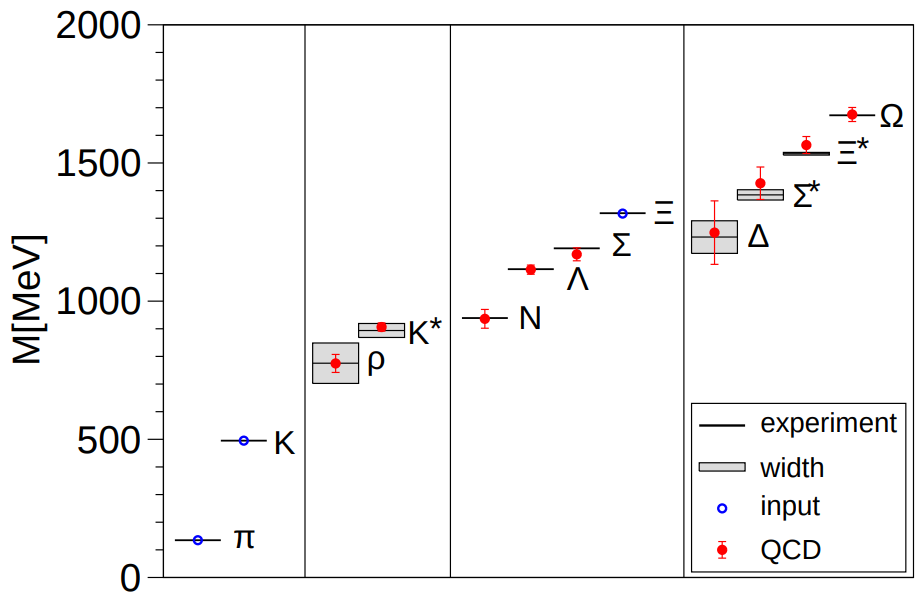
\includegraphics[width=0.7\linewidth]{Figures/Chapter 1/LQCD_hadron_mass.png}
  \caption{The light hadron spectrum of QCD. Horizontal lines and bands are the experimental values with their decay widths. Lattice QCD results~\cite{BMW:2008jgk} are shown by solid circles. Vertical error bars represent the combined statistical and systematic error estimates. $\pi$, K and $\Xi$ have no error bars, because they are used to set the light quark mass, the strange quark mass, and the overall scale, respectively.}
  \label{fig:LQCD_hadron_mass}
\end{figure}

\section{Quark Gluon Plasma}
The concept of deconfinement refers to the transition from a confined state to a state where quarks and gluons are no longer confined within hadrons, but are free to move in a larger volume. As modelled by the MIT bag model, non-perturbative QCD effects can be described in terms of an external pressure, which confines quarks and gluons within a finite volume. If the external pressure is overcome by the pressure due to the kinematic energy of the quarks and gluons, then the hadrons constituents are no longer confined, and a transition to a state called Quark-Gluon Plasma (QGP) occurs. Lattice QCD calculations are used to understand the properties of the QGP, and they predict that a strongly interacting system with zero net baryon density evolves smoothly from a confined (hadronic) towards a deconfined (quarks and gluons) state when its temperature is increased up to $\sim155$ MeV ($1.8\times 10^12$ K)~\cite{HotQCD:2014kol, Borsanyi:2013bia}. During the transition, both deconfined and hadronic matter can exist, and the transition is called a crossover.

\begin{figure}
  \centering
  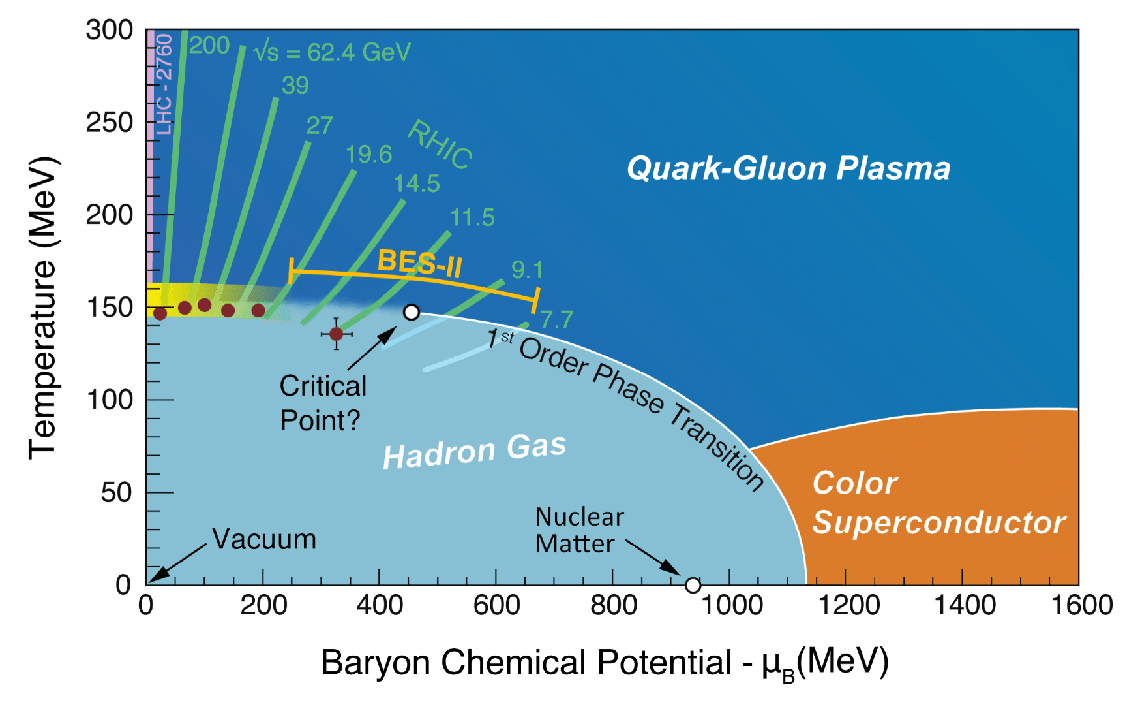
\includegraphics[width=0.7\linewidth]{Figures/Chapter 1/QCD-diagram.jpg}
  \caption{QCD phase diagram in the temperature-baryon chemical potential plane.}
  \label{fig:PhaseDiagram}
\end{figure}

It is believed that the universe underwent a phase of deconfinement in the early stages of its evolution, a few microseconds after the Big Bang. Direct observation of the primordial QGP (i.e. that created just after the Big Bang) would provide a wealth of information on the early universe; however, the universe experienced a phase in which electrons were not bound to nuclei, making it opaque to electromagnetic radiation, and denying us the possibility of directly observing the QGP. Once the universe cooled enough (3000~K) to allow electrons to bind to nuclei, the electromagnetic radiation decoupled with a black body spectrum of around 3000 K. Since then, as the universe expanded, this electromagnetic radiation has redshifted to a temperature of around 2.7~K, and is denoted as the Cosmic Microwave Background (CBM). The CMB is the oldest light in the universe and provides a snapshot of the universe when it was 300,000 years old, long after the QGP had already cooled down. Hence, the only way to study the QGP is by recreating it in the laboratory, through the collision of heavy ions at high energies. In the past decades, several experiments~\cite{ALICE:2022wpn, NA38:2000wlp, NA50:1997hlx, Nouicer:2009fy} have been carried out to study the properties of this state of matter, and the results have provided valuable insights into the properties of the strong interaction at high energy scales.

\subsection{Heavy-ion collisions}
Heavy-ion collisions are the most suitable environment to study the properties of the QGP. In these collisions, two heavy ions, such as lead or gold nuclei, are accelerated to ultra-relativistic energies and made to collide head-on. Given the large amount of energy deposited in the collision, the system reaches high energy densities of around 16 GeV/fm$^3$ after 1 fm/$c$~\cite{Loizides:2011ys}, which allows for the production of the QGP. As nuclei are objects made many nucleons (i.e. protons and neutrons), the interaction volume (called \emph{fireball}) is larger and longer-lived than in proton-proton collisions, allowing to use thermodynamics and fluidodynamics to describe the system. 

The collision of two nuclei is a rather complex process, with a space-time evolution that can be divided into several stages. It is possible to distinguish between two different collision regimes. When the centre-of-mass energy per nucleon pair (\snn) is below a few GeV, the nucleons are stopped in the collision as they lose energy and momentum. Due to conserved currents, the quantum numbers of the initial state are preserved, so that, for example, the net baryon production (i.e. the difference between the number of baryons and antibaryons) is positive. This regime is called \emph{stopping regime}. When the \snn increases, the initial state baryon number is carried away by the receding nucleons, and the net baryon number in the fireball is zero. This regime is denoted as \emph{Bjorken regime}, or \emph{transparency regime}. When the \snn is above a few GeV, the collision is dominated by the interaction of the partons in the colliding nuclei, and the system is described as a collection of quarks and gluons.

The initial stage is characterised by the collision of the two nuclei, which leads to the formation of a fireball. The fireball expands and cools down, and the quarks and gluons are deconfined, leading to the formation of the QGP. The QGP expands and cools down further, and eventually hadronises, leading to the formation of hadrons. The hadrons interact with each other and with the surrounding medium, and they are detected in the final state. The study of the properties of the QGP is performed by measuring the hadrons produced in the final state, and by studying their properties, such as their momentum spectra, their azimuthal correlations, and their mass distributions. The results of the experiments are compared to theoretical models, such as hydrodynamics and transport models, to extract information on the properties of the QGP.

\begin{figure}[htb]
  \centering
  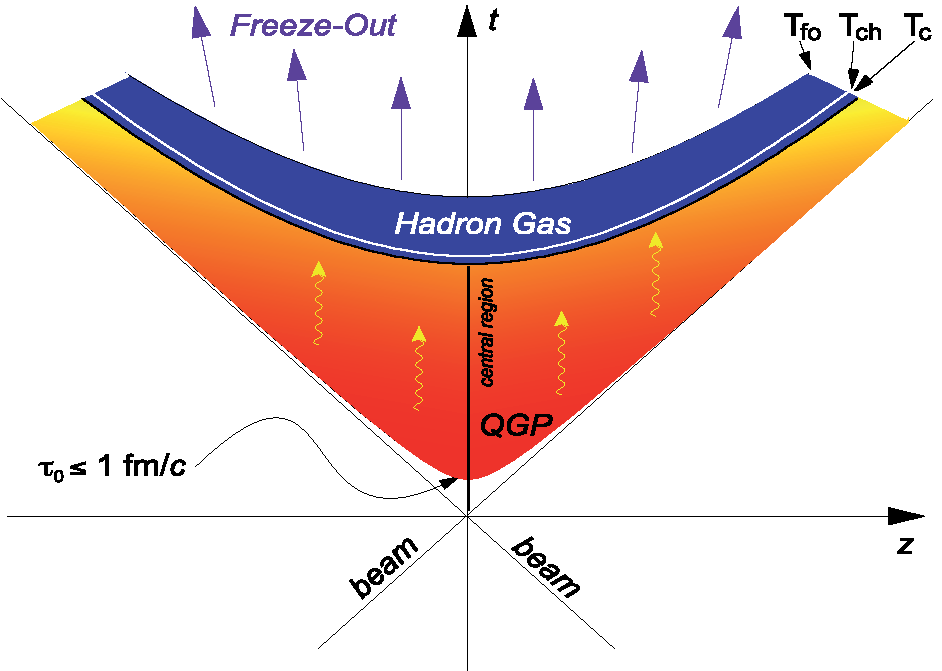
\includegraphics[width=0.7\linewidth]{Figures/Chapter 1/Bild_18.pdf}
  \caption{Schematic view of a heavy-ion collision.}
  \label{fig:HeavyIonCollisions}
\end{figure}


\section{Strangenness enhancement}
One of the first proposed signatures of the QGP formation is the strangeness enhancement~\cite{Rafelski:1982pu}, which refers to the observation of an increased production of strange hadrons in heavy-ion collisions compared to proton-proton collisions. At a microscopic level, the enhancement of strange hadrons is a direct consequence of the high energy densities reached in the collisions, which allow for the thermal production of strange quarks and antiquarks. Strange quarks are not present as valence quarks in the initial state, and can be produced in hard $2\rightarrow 2$ scatterings ($gg\rightarrow s\overline{s}, q\overline{q}\rightarrow s\overline{s}$), or via gluon splitting ($g\rightarrow s\overline{s}$) during the evolution of the system. While these processes are dominant for the production of strange hadrons with high \pt, at low \pt the production of strange hadrons is dominated by non-perturbative processes. At a macroscopic level, the enhancement of the production of strange hadrons can be explained using a statistical approach, in a framework known as the statistical hadronisation model. In this model, the system is described as an ideal gas of hadrons and resonances, which is assumed to be in thermal and chemical equilibrium at the chemical freeze-out. The hadrons production in heavy-ion collisions is described according to a grand-canonical ensemble statistical distribution, which depends on the temperature and the chemical potentials of the system. In a grand-canonical ensemble, which is used to describe a system that exchanges both energy and particles with a reservoir, the energy and quantum numbers are only conserved on average on a large volume. The description of the hadrons production in smaller colliding systems, such as $\mathrm{e^+e^-}$ and pp collisions, requires the use of a canonical ensemble, which is used to describe a system that exchanges only energy with a reservoir, and requires the exact (local) conservation of the quantum numbers. This leads to a suppression of strange quark production as compared to the grand canonical ensemble. 

The strangeness enhancement in heavy-ion collisions has been observed in several experiments, such as the STAR experiment at RHIC~\cite{STAR:2007cqw} and the ALICE experiment at the LHC~\cite{ALICE:2013xmt}. In addition, an enhancement of strange hadrons has been observed in small systems, such as pp~\cite{ALICE:2016fzo} and p-Pb~\cite{ALICE:2013wgn, ALICE:2015mpp} collisions, in high-multiplicity events, and follows a hierarchy determined by the hadron strangeness. This observation is intriguing, as QGP production is not expected in such systems. Furthermore, several effects such as azimuthal correlations and mass-dependent hardening of \pt distributions, which are typically associated with QGP formation in nuclear collisions, have been observed in these systems. Could small droplets of QGP be formed in these collisions? Could other mechanisms explain the observed effects? These are still open questions in the field of high-energy nuclear physics, and they are the subjects of ongoing research.

Figure~\ref{fig:StrangenessEnhancement} shows the \pt-integrated yield ratios of strange (\kzs, $\Lambda$) and multi-strange ($\Xi^\pm, \Omega^\pm$) hadrons to pions ($\pi^++\pi^-$) as a function of the charged particle multiplicity density, $\braket{\de N_\mathrm{ch}/\de\eta}$, measured in $\lvert y\rvert<0.5$ in different collision systems (pp, p--Pb and Pb--Pb) using the ALICE experiment at the LHC~\cite{ALICE:2016fzo}. The data show a clear enhancement of strange to non-strange hadron production with increasing multiplicity. At the highest multiplicities, the yield ratios saturate at values that are compatible with what is measured in central Pb-Pb collisions, where QGP is formed.

\begin{figure}[htb!]
  \centering
  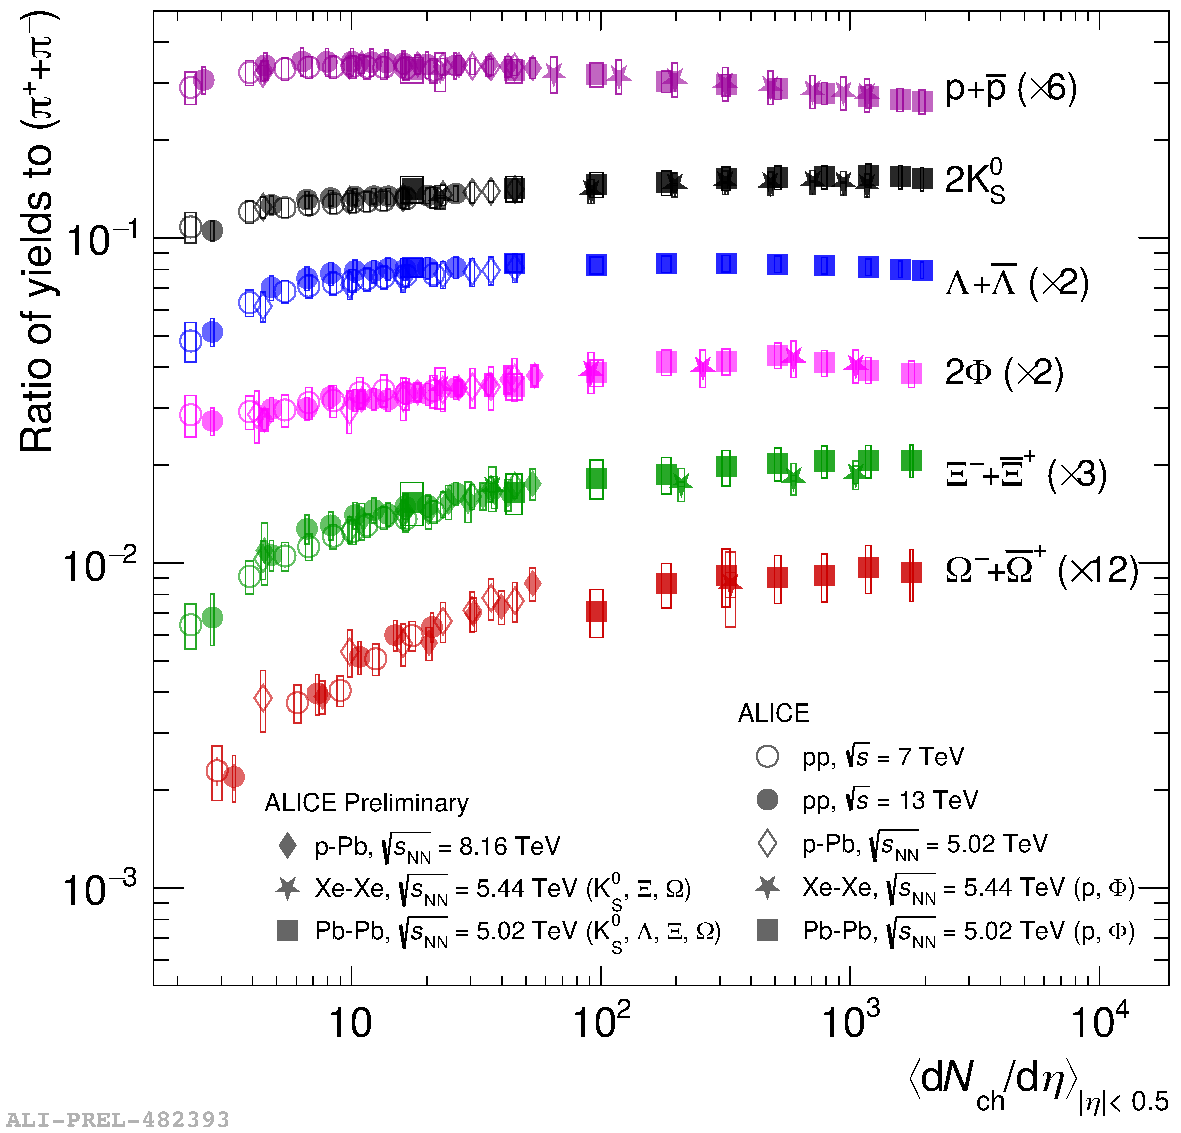
\includegraphics[width=0.5\linewidth]{Figures/Chapter 1/img_ToPionRatios_1.pdf}
  \caption{\pt--integrated yield ratios of strange (\kzs, $\Lambda$) and multi-strange ($\Xi^\pm, \Omega^\pm$) hadrons to pions ($\pi^++\pi^-$) as a function of $\braket{\de N_\mathrm{ch}/\de\eta}$ measured in pp, p--Pb and Pb--Pb collisions at midrapidity$(\lvert y\rvert<0.5)$.}
  \label{fig:StrangenessEnhancement}
\end{figure}


%In the QGP, strange quarks are produced through the interactions between the quarks and gluons, and they can form strange hadrons, such as the $\Lambda$, $\Xi$, and $\Omega$ baryons. The production of strange hadrons in heavy-ion collisions is a key signature of the QGP, and it has been observed in several experiments, such as the ALICE experiment at the LHC~\cite{ALICE:2022wpn}. The strangeness enhancement is a direct consequence of the high energy densities reached in the collisions, which allow for the production of strange quarks and antiquarks. In the QGP, strange quarks are produced through the interactions between the quarks and gluons, and they can form strange hadrons, such as the $\Lambda$, $\Xi$, and $\Omega$ baryons. The production of strange hadrons in heavy-ion collisions is a key signature of the QGP, and it has been observed in several experiments, such as the ALICE experiment at the LHC~\cite{ALICE:2022wpn}.